% !TEX root = ../main.tex
\section{Laser Diode}
\label{sec:laser_diode}

The earliest semiconductor lasers were homojunction lasers, which were
demonstrated in 1962. These “proof of concept” lasers featured a threshold
current density of $\SI{19000}{A/cm^{2}}$ at cryogenic temperature. A prominent vertical
layer structure that was realized in 1969–1970 is the Double Heterostructure. In
comparison to homojunctions, a double heterostructure (DHS) featured a significantly
lower threshold current density ($\SI{1600}{A/cm^{2}}$) and could be operated at room
temperature.

However, almost all commercial laser diodes today are no longer simple double-heterostructure
lasers but quantum-well lasers, usually with a separate-confinement heterostructure
(SCH). The first single and multiple quantum-well lasers were demonstrated in
1977 by Holonyak’s group using liquid-phase epitaxy. Confining the electron-hole pairs
to the thin well region reduced the threshold current density to about $\SI{500}{A/cm^{2}}$.
Introducing strain into the quantum wells in the late 1980s lowered it further
to $\SI{65}{A/cm^{2}}$ at room temperature.

\subsection{Vertical Structure}
\label{sec:vertical_structure}

A thin layer of low-band-gap material is embedded between two layers of higher-band-gap
material. See \cref{fig:double_heterostructure}. The band-gap step confines
charge carriers and the refractive-index step confines light, both in the same thin
layer. A popular material system is $\ce{GaAs}$ as gain medium with
$\ce{AlGaAs}$ as cladding.

\begin{figure}
	\centering
	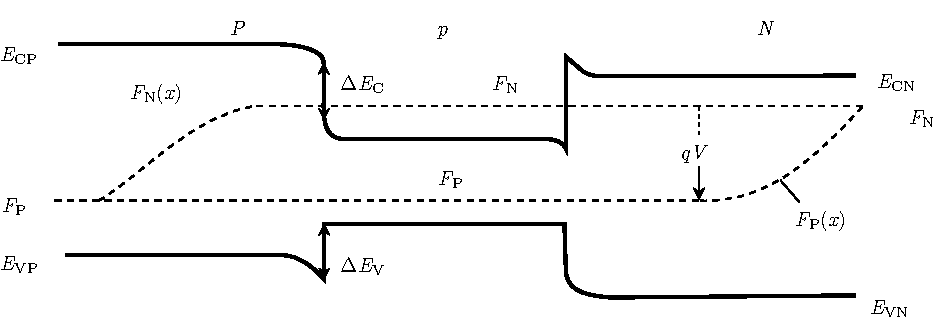
\includegraphics[width=\linewidth]{../assets/band_diagram.pdf}
	\caption{Band diagram of a $P$-$p$-$N$ double heterostructure under forward
	bias $V$. \imcite{chuang_physics_2009}}
	\label{fig:double_heterostructure}
\end{figure}

The band offsets form potential wells that trap injected charge carriers in the low-gap
layer, where they recombine. However, carriers with an energy higher than the
barrier height can pass over the barrier, escape from the well and no longer recombine
in the active layer. This effect results in a leakage current $I_{\mathrm{L}}$.

In the transparent regime, $\epsilon'' \simeq 0$ and $n_{\mathrm{r}}\simeq \sqrt{
\epsilon'}$. Using the oscillator model:
\begin{equation}
	\epsilon'=1 + \int \frac{e^{2}}{\epsilon_{0}m_{0}\omega_{\mathrm{cv}}^{2}}\frac{2
	\lvert \mathbf{p}_{\mathrm{cv}}\rvert^{2}}{m_{0}\hbar \omega_{\mathrm{cv}}}\frac{1}{1-\omega^{2}/\omega_{\mathrm{cv}}^{2}}
	\, \frac{\mathrm{d}\mathbf{k}}{(2\pi)^{3}}
\end{equation}

% \begin{table}[H]
% \centering
% \begin{tabular}{p{0.32\textwidth}p{0.32\textwidth}p{0.32\textwidth}}
% \toprule
% Symbol & Meaning & Unit \\
% \midrule
% $\epsilon'$ & real part of the relative dielectric function & dimensionless \\
% $e$ & elementary charge & $\mathrm{C}$ \\
% $\epsilon_{0}$ & vacuum permittivity & $\mathrm{F\,m^{-1}}$ \\
% $m_{0}$ & free electron mass & $\mathrm{kg}$ \\
% $\omega_{\mathrm{cv}}$ & angular frequency of the interband transition at $\mathbf{k}$, $\hbar\omega_{\mathrm{cv}}=E_{\mathrm{c}}(\mathbf{k})-E_{\mathrm{v}}(\mathbf{k})$ & $\mathrm{rad\,s^{-1}}$ \\
% $\mathbf{p}_{\mathrm{cv}}$ & momentum matrix element between conduction- and valence-band states & $\mathrm{kg\,m\,s^{-1}}$ \\
% $\hbar$ & reduced Planck constant & $\mathrm{J\,s}$ \\
% $\omega$ & angular frequency of the light & $\mathrm{rad\,s^{-1}}$ \\
% $\mathbf{k}$ & wavevector of the electronic states & $\mathrm{m^{-1}}$ \\
% \bottomrule
% \end{tabular}
% \caption{TODO}
% \end{table}

If the band-gap energy decreases, $\omega_{\mathrm{cv}}$ decreases, so that all factors
of the integrand increase. Hence, both $\epsilon'$ and $n_{\mathrm{r}}$ increase.
A low-gap layer consequently has a higher refractive index than its surroundings,
leading to wave guiding in this layer. The layer acts like the core of a glass
fiber in which light is guided (see \cref{fig:refractive_index_profile}).

\begin{figure}[H]
	\centering
	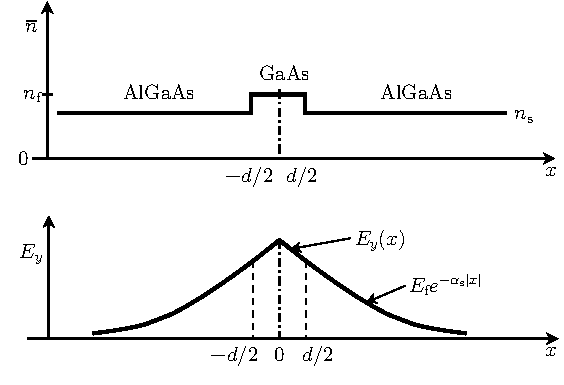
\includegraphics[width=0.6\linewidth]{../assets/refractive_index_profile.pdf}
	\caption{Profile of the refractive index $\bar n$ of an AlGaAs/GaAs double
	heterostructure (top) with the core index $n_{\mathrm{f}}$ and the cladding
	index $n_{\mathrm{s}}$, and approximate field distribution $E_{y}(x)$ of the guided
	optical wave (bottom). The field is approximated by an exponential decay
	$E_{\mathrm{f}}e^{-\alpha_{\mathrm{s}}\lvert x\rvert}$ with the peak amplitude
	$E_{\mathrm{f}}$ and the decay constant $\alpha_{\mathrm{s}}$ in the cladding. \imcite{ebeling_integrated_1993}}
	\label{fig:refractive_index_profile}
\end{figure}

% Gliederung: [[Optical Confinement Factor]]
% ---- Optical Confinement Factor.md ----

A key metric is the Optical Confinement Factor $\Gamma$. It is the fraction of the
light intensity, integrated over the cross section, that lies within a specified region.
For a one-dimensional problem in which the specified region is centered at the
origin and has the width $d$, $\Gamma$ can be expressed as:
\begin{equation}
	\Gamma=\frac{\int_{-d /2}^{d /2}\lvert E(x) \rvert^{2}\, \mathrm{d}x}{\int_{-\infty}^{\infty}\lvert
	E(x) \rvert^{2}\, \mathrm{d}x}
\end{equation}

% \begin{table}[H]
% \centering
% \begin{tabular}{p{0.32\textwidth}p{0.32\textwidth}p{0.32\textwidth}}
% \toprule
% Symbol & Meaning & Unit \\
% \midrule
% $\Gamma$ & optical confinement factor & dimensionless \\
% $E$ & electric field amplitude of the guided mode & $\mathrm{V\,m^{-1}}$ \\
% $x$ & position perpendicular to the layers & $\mathrm{m}$ \\
% $d$ & width of the specified region (e.g. active layer thickness) & $\mathrm{m}$ \\
% \bottomrule
% \end{tabular}
% \caption{TODO}
% \end{table}

The confinement factor of the gain region is used as a figure of merit in laser
diodes. A value of $\Gamma$ close to one is desirable.

\subsection{Lateral Structure}
\label{sec:lateral_structure}

% Gliederung: [[Laser Diode]]: Abschnitte zur Schichtstruktur und lateralen Struktur (Gain Guiding, Index Guiding)
% ---- Laser Diode.md ----

The lateral structure confines current and light in the direction parallel to
the layers; the two common approaches are gain guiding and index guiding (see
\cref{fig:gain_index_guiding}).

To achieve a high current density at low external currents, the current is
injected only into a narrow stripe. For this purpose, the surface contact is
insulated by an oxide layer everywhere except for a narrow stripe running
parallel to the cavity. Since optical gain only occurs where carriers are injected,
the current density profile also determines the lateral extension of the light
wave. This mechanism is known as “gain guiding”.

In a ridge waveguide structure, the p-type layer is etched away except for a
small stripe, the so-called mesa. As a result, the effective thickness of the p-AlGaAs
cladding layer differs between the region below the mesa and its surroundings,
which changes the effective refractive index. Since the effective refractive index
is higher below the mesa, the wave is guided in this region. This mechanism is known
as “index guiding”.

\begin{figure}[H]
	\centering
	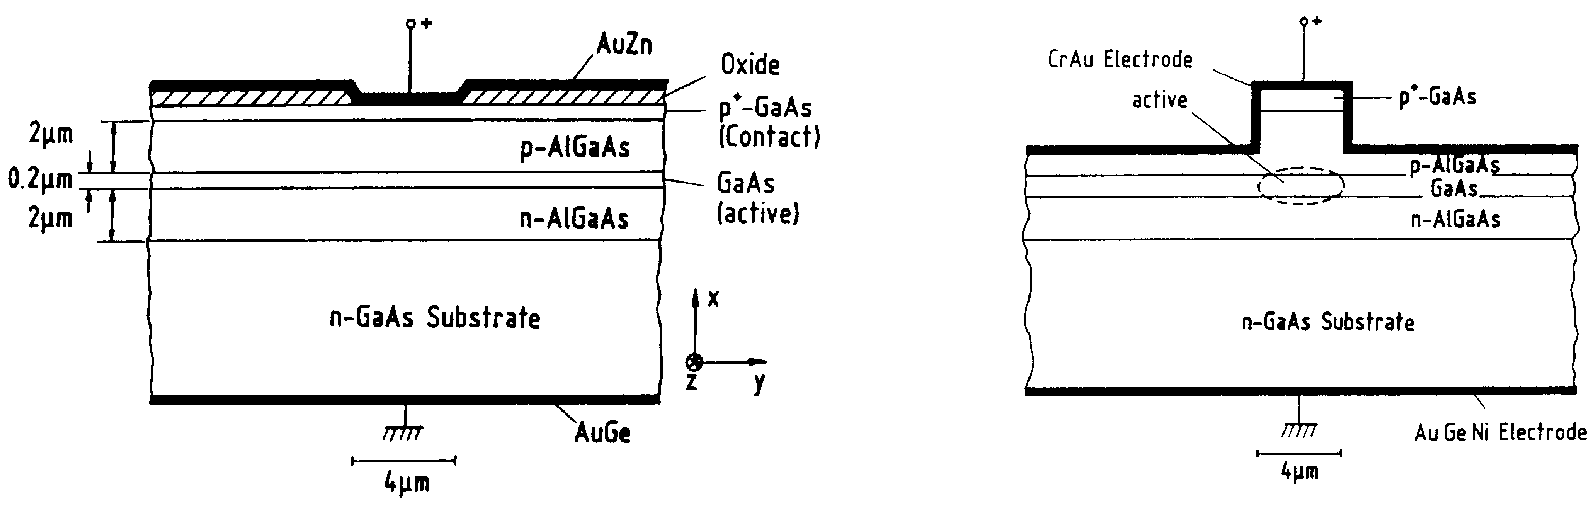
\includegraphics[width=\linewidth]{../assets/gain_index_guiding.png}
	\caption{Cross section of an oxide stripe laser (left) as an example for gain
	guiding and a ridge waveguide laser (right) as an example for index guiding. \imcite{ebeling_integrated_1993}}
	\label{fig:gain_index_guiding}
\end{figure}

\subsection{Resonator and Threshold}
\label{sec:resonator_and_threshold}

% Gliederung: [[Fabry-Perot Resonator]]
% ---- Fabry-Perot Resonator.md ----

A crucial part of a laser is a resonator that feeds part of the light back into the
amplifying medium. This resonator consists of two plane-parallel mirrors. In semiconductor
lasers, the mirrors are realized as smooth cleaved facets at both ends of the
active stripe. A laser oscillates when a light wave returns after one round trip with
identical amplitude and phase. The gain must then exactly compensate all losses.

The cleaved facets act as mirrors through Fresnel reflection at the
semiconductor–air interface; at normal incidence, the reflectivity is:
\begin{equation}
	R=\left(\frac{\bar n-1}{\bar n+1}\right)^{2}
\end{equation}

% \begin{table}[H]
% \centering
% \begin{tabular}{p{0.32\textwidth}p{0.32\textwidth}p{0.32\textwidth}}
% \toprule
% Symbol & Meaning & Unit \\
% \midrule
% $R$ & intensity reflectivity of a cleaved facet & dimensionless \\
% $\bar n$ & effective refractive index of the mode & dimensionless \\
% \bottomrule
% \end{tabular}
% \caption{TODO}
% \end{table}

\subsubsection{Round-Trip Condition}

The light intensity of the guided mode grows with the modal gain $\Gamma g$ and
decays with the intrinsic loss $\alpha_{\mathrm{i}}$. As the electric field amplitude
scales with the square root of the intensity, it varies along the cavity as:
\begin{equation}
	E(z)=E_{0}\exp\left[\tfrac{1}{2}(\Gamma g-\alpha_{\mathrm{i}})z\right]\exp(\mathrm{i}
	\beta z),\qquad \beta=\frac{2\pi\bar n}{\lambda}
\end{equation}

% \begin{table}[H]
% \centering
% \begin{tabular}{p{0.32\textwidth}p{0.32\textwidth}p{0.32\textwidth}}
% \toprule
% Symbol & Meaning & Unit \\
% \midrule
% $E(z), E_0$ & electric field amplitude of the mode along the cavity / at $z=0$ & $\mathrm{V\,m^{-1}}$ \\
% $z$ & position along the cavity axis & $\mathrm{m}$ \\
% $\Gamma$ & optical confinement factor & dimensionless \\
% $g$ & material gain coefficient & $\mathrm{m^{-1}}$ \\
% $\alpha_{\mathrm i}$ & intrinsic loss & $\mathrm{m^{-1}}$ \\
% $\beta$ & propagation constant of the mode & $\mathrm{m^{-1}}$ \\
% $\bar n$ & effective refractive index of the mode & dimensionless \\
% $\lambda$ & vacuum wavelength & $\mathrm{m}$ \\
% \bottomrule
% \end{tabular}
% \caption{TODO}
% \end{table}

The intrinsic loss $\alpha_{\mathrm{i}}$ originates from free-carrier absorption in
the waveguide materials and from scattering at rough waveguide walls. At each
facet only the fraction $r_{1}$ or $r_{2}$ of the field amplitude is reflected. After
a round trip (length $2L$, two reflections) the field has to reproduce itself:
\begin{equation}
	r_{1} r_{2}\,\exp\left[(\Gamma g-\alpha_{\mathrm{i}})L\right]\exp(2\mathrm{i}\beta
	L)=1
\end{equation}

% \begin{table}[H]
% \centering
% \begin{tabular}{p{0.32\textwidth}p{0.32\textwidth}p{0.32\textwidth}}
% \toprule
% Symbol & Meaning & Unit \\
% \midrule
% $r_1, r_2$ & amplitude reflection coefficients of the two facets, $R_{1,2}=\lvert r_{1,2}\rvert^2$ & dimensionless \\
% $\Gamma$ & optical confinement factor & dimensionless \\
% $g$ & material gain coefficient & $\mathrm{m^{-1}}$ \\
% $\alpha_{\mathrm i}$ & intrinsic loss & $\mathrm{m^{-1}}$ \\
% $L$ & length of the laser cavity & $\mathrm{m}$ \\
% $\beta$ & propagation constant of the mode & $\mathrm{m^{-1}}$ \\
% \bottomrule
% \end{tabular}
% \caption{TODO}
% \end{table}

As this condition is complex-valued, it splits into one condition for the
magnitude (threshold) and one for the phase (modes).

\paragraph{Amplitude Condition: Threshold}

Since the reflectivities $R_{1/2}$ refer to intensities, the amplitude reflection
coefficients are their square roots, $r_{1}r_{2}=\sqrt{R_{1}R_{2}}$. The magnitude
of the round-trip condition fixes the gain needed at threshold:
\begin{equation}
	\sqrt{R_{1}R_{2}}\,\exp\left[(\Gamma g_{\mathrm{th}}-\alpha_{\mathrm{i}})L\right
	]\overset{!}{=}1 \quad\Rightarrow\quad \Gamma g_{\mathrm{th}}=\alpha_{\mathrm{i}}
	+\underbrace{\frac{1}{2L}\ln\frac{1}{R_{1}R_{2}}}_{\alpha_{\mathrm{m}}}=\alpha_{\mathrm{i}}
	+\alpha_{\mathrm{m}}
\end{equation}
% \begin{table}[H]
% \centering
% \begin{tabular}{p{0.32\textwidth}p{0.32\textwidth}p{0.32\textwidth}}
% \toprule
% Symbol & Meaning & Unit \\
% \midrule
% $R_1, R_2$ & intensity reflectivities of the two facets & dimensionless \\
% $\Gamma$ & optical confinement factor & dimensionless \\
% $g_{\mathrm{th}}$ & gain coefficient at threshold & $\mathrm{m^{-1}}$ \\
% $\alpha_{\mathrm i}$ & intrinsic loss & $\mathrm{m^{-1}}$ \\
% $\alpha_{\mathrm m}$ & mirror loss & $\mathrm{m^{-1}}$ \\
% $L$ & length of the laser cavity & $\mathrm{m}$ \\
% \bottomrule
% \end{tabular}
% \caption{TODO}
% \end{table}
The mirror loss $\alpha_{\mathrm{m}}$ accounts for the light leaving through the
facets, which forms the useful laser output. At threshold, the modal gain balances
the intrinsic and mirror losses.

\paragraph{Phase Condition: Longitudinal Modes}

The phase of the round-trip condition has to be a multiple of $2\pi$:
\begin{equation}
	2\beta L\overset{!}{=}2\pi m\quad\Rightarrow\quad m\lambda=2L\bar n
\end{equation}
% \begin{table}[H]
% \centering
% \begin{tabular}{lll}
% \toprule
% Symbol & Meaning & Unit \\
% \midrule
% $m$ & longitudinal mode number & dimensionless (integer) \\
% $\beta$ & propagation constant of the mode & $\mathrm{m^{-1}}$ \\
% $L$ & length of the laser cavity & $\mathrm{m}$ \\
% $\lambda$ & vacuum wavelength & $\mathrm{m}$ \\
% $\bar n$ & effective refractive index of the mode & dimensionless \\
% \bottomrule
% \end{tabular}
% \caption{TODO}
% \end{table}
The amplitude condition decides whether a mode lases, and the phase condition at which
wavelength it lases. Using finite difference approximation as
$\Delta m /\Delta\lambda \simeq \partial_{\lambda}m$, the mode separation for large
$m$ is given as:
\begin{equation}
	\Delta\lambda=\frac{\lambda^{2}\Delta m}{2\bar{n}L[1-(\lambda /\bar{n})(\mathrm{d}\bar{n}/\mathrm{d}\lambda)]}
\end{equation}

% \begin{table}[H]
% \centering
% \begin{tabular}{p{0.32\textwidth}p{0.32\textwidth}p{0.32\textwidth}}
% \toprule
% Symbol & Meaning & Unit \\
% \midrule
% $\Delta\lambda$ & wavelength spacing between modes & $\mathrm{m}$ \\
% $\Delta m$ & difference in mode number & dimensionless (integer) \\
% $\lambda$ & vacuum wavelength & $\mathrm{m}$ \\
% $\bar n$ & effective refractive index of the mode & dimensionless \\
% $\mathrm{d}\bar n/\mathrm{d}\lambda$ & dispersion of the effective refractive index & $\mathrm{m^{-1}}$ \\
% $L$ & length of the laser cavity & $\mathrm{m}$ \\
% \bottomrule
% \end{tabular}
% \caption{TODO}
% \end{table}

\subsection{P-I Characteristic}
\label{sec:p_i_characteristic}

% Gliederung: [[Laser Diode P-I Curve]]: verwendet $\Gamma$, $\alpha_{\mathrm m}$, $g_{\mathrm{th}}$ und $I_{\mathrm L}$ aus den vorherigen Abschnitten
% ---- Laser Diode P-I Curve.md ----

A rate equation can be used to
describe the dynamics of the carrier density $n$ and the Photon Density $S$:
\begin{equation}
	\frac{\mathrm{d}n(t)}{\mathrm{d}t}= \eta_{\mathrm{i}}\frac{j(t)}{qd}- R(n) - v_{\mathrm{g}}
	g(n) S(t)
\end{equation}

% \begin{table}[H]
% \centering
% \begin{tabular}{lll}
% \toprule
% Symbol & Meaning & Unit \\
% \midrule
% $n$ & carrier density & $\mathrm{m^{-3}}$ \\
% $t$ & time & $\mathrm{s}$ \\
% $\eta_{\mathrm i}$ & collection efficiency & dimensionless \\
% $j$ & injection current density & $\mathrm{A\,m^{-2}}$ \\
% $q$ & elementary charge & $\mathrm{C}$ \\
% $d$ & thickness of the active region & $\mathrm{m}$ \\
% $R(n)$ & recombination rate per volume & $\mathrm{m^{-3}\,s^{-1}}$ \\
% $v_{\mathrm g}$ & group velocity of the light & $\mathrm{m\,s^{-1}}$ \\
% $g(n)$ & material gain coefficient & $\mathrm{m^{-1}}$ \\
% $S$ & photon density & $\mathrm{m^{-3}}$ \\
% \bottomrule
% \end{tabular}
% \caption{TODO}
% \end{table}

The first term on the right hand side describes the carrier injection into the active region with
thickness $d$ and collection efficiency $\eta_{\mathrm{i}}$. $R(n)$ represents (radiative
and nonradiative) recombination processes. The last term expresses the carrier
loss due to stimulated emission.

Using the ABC model, the recombination rate is given as:
\begin{align}
	R(n)    & =An +Bn^{2}+Cn^{3}=\frac{n}{\tau(n)} \\
	\tau(n) & =(A+Bn+Cn^{2})^{-1}
\end{align}
% \begin{table}[H]
% \centering
% \begin{tabular}{p{0.32\textwidth}p{0.32\textwidth}p{0.32\textwidth}}
% \toprule
% Symbol & Meaning & Unit \\
% \midrule
% $R(n)$ & recombination rate per volume & $\mathrm{m^{-3}\,s^{-1}}$ \\
% $\tau(n)$ & carrier lifetime & $\mathrm{s}$ \\
% $n$ & carrier density & $\mathrm{m^{-3}}$ \\
% $A, B, C$ & coefficients for defect, radiative and Auger recombination & $\mathrm{s^{-1}}$, $\mathrm{m^{3}\,s^{-1}}$, $\mathrm{m^{6}\,s^{-1}}$ \\
% \bottomrule
% \end{tabular}
% \caption{TODO}
% \end{table}
where $An$ represents nonradiative recombination of carriers with defects, $Bn^{2}$
the spontaneous emission and $Cn^{3}$ the nonradiative Auger recombination.

\paragraph{Steady State with Low Current Density}

In steady state and at low current density, the carrier concentration is determined
by the injection current. As the photon density is negligible ($S \simeq 0$), it follows
that:
\begin{equation}
	\eta_{\mathrm{i}}\frac{j}{qd}=\frac{n}{\tau}
\end{equation}

% \begin{table}[H]
% \centering
% \begin{tabular}{lll}
% \toprule
% Symbol & Meaning & Unit \\
% \midrule
% $\eta_{\mathrm i}$ & collection efficiency & dimensionless \\
% $j$ & injection current density & $\mathrm{A\,m^{-2}}$ \\
% $q$ & elementary charge & $\mathrm{C}$ \\
% $d$ & thickness of the active region & $\mathrm{m}$ \\
% $n$ & carrier density & $\mathrm{m^{-3}}$ \\
% $\tau$ & carrier lifetime & $\mathrm{s}$ \\
% \bottomrule
% \end{tabular}
% \caption{TODO}
% \end{table}

The carrier density $n$ can be obtained by assuming either a constant $\tau$ or
constant $A, B, C$ parameters. Typically, a linear relation for the peak gain
coefficient versus carrier density is assumed using the differential gain $g'$
and the transparency concentration $n_{\mathrm{tr}}$:
\begin{equation}
	g(n)=g' (n-n_{\mathrm{tr}})
\end{equation}

% \begin{table}[H]
% \centering
% \begin{tabular}{lll}
% \toprule
% Symbol & Meaning & Unit \\
% \midrule
% $g(n)$ & peak material gain coefficient & $\mathrm{m^{-1}}$ \\
% $g'$ & differential gain & $\mathrm{m^{2}}$ \\
% $n$ & carrier density & $\mathrm{m^{-3}}$ \\
% $n_{\mathrm{tr}}$ & transparency carrier density & $\mathrm{m^{-3}}$ \\
% \bottomrule
% \end{tabular}
% \caption{TODO}
% \end{table}

\paragraph{Threshold Condition}

The round-trip condition that is enforced in a Fabry-Perot Resonator (see \cref{sec:resonator_and_threshold}) results in
a threshold condition of the material gain:
\begin{equation}
	\Gamma g_{\mathrm{th}}=\alpha_{\mathrm{i}}+\alpha_{\mathrm{m}}
\end{equation}

% \begin{table}[H]
% \centering
% \begin{tabular}{lll}
% \toprule
% Symbol & Meaning & Unit \\
% \midrule
% $\Gamma$ & optical confinement factor & dimensionless \\
% $g_{\mathrm{th}}$ & gain coefficient at threshold & $\mathrm{m^{-1}}$ \\
% $\alpha_{\mathrm i}$ & intrinsic loss & $\mathrm{m^{-1}}$ \\
% $\alpha_{\mathrm m}$ & mirror loss & $\mathrm{m^{-1}}$ \\
% \bottomrule
% \end{tabular}
% \caption{TODO}
% \end{table}

The modal gain $\Gamma
g_{\mathrm{th}}$ must equal the sum of the intrinsic loss $\alpha_{\mathrm{i}}$ and
the mirror loss $\alpha_{\mathrm{m}}$. With increasing $j$, $n$ increases and therefore
$g$ increases up to its threshold value. Consequently, $g_{\mathrm{th}}$ limits $n$
to $n_{\mathrm{th}}$, which is reached for $j=j_{\mathrm{th}}$.
\begin{align}
	g_{\mathrm{th}} & =\frac{\alpha_{\mathrm{i}}+\alpha_{\mathrm{m}}}{\Gamma}                                   \\
	n_{\mathrm{th}} & =n_{\mathrm{tr}}+(\alpha_{\mathrm{i}}+\alpha_{\mathrm{m}}) /(\Gamma g')                   \\
	j_{\mathrm{th}} & =\frac{qd}{\eta_{\mathrm{i}}}(An_{\mathrm{th}}+Bn_{\mathrm{th}}^{2}+Cn_{\mathrm{th}}^{3}) \label{eq:j_th}
\end{align}

% \begin{table}[H]
% \centering
% \begin{tabular}{p{0.32\textwidth}p{0.32\textwidth}p{0.32\textwidth}}
% \toprule
% Symbol & Meaning & Unit \\
% \midrule
% $g_{\mathrm{th}}$ & gain coefficient at threshold & $\mathrm{m^{-1}}$ \\
% $\alpha_{\mathrm i}$ & intrinsic loss & $\mathrm{m^{-1}}$ \\
% $\alpha_{\mathrm m}$ & mirror loss & $\mathrm{m^{-1}}$ \\
% $\Gamma$ & optical confinement factor & dimensionless \\
% $n_{\mathrm{th}}$ & carrier density at threshold & $\mathrm{m^{-3}}$ \\
% $n_{\mathrm{tr}}$ & transparency carrier density & $\mathrm{m^{-3}}$ \\
% $g'$ & differential gain & $\mathrm{m^{2}}$ \\
% $j_{\mathrm{th}}$ & threshold current density & $\mathrm{A\,m^{-2}}$ \\
% $q$ & elementary charge & $\mathrm{C}$ \\
% $d$ & thickness of the active region & $\mathrm{m}$ \\
% $\eta_{\mathrm i}$ & collection efficiency & dimensionless \\
% $A, B, C$ & coefficients for defect, radiative and Auger recombination & $\mathrm{s^{-1}}$, $\mathrm{m^{3}\,s^{-1}}$, $\mathrm{m^{6}\,s^{-1}}$ \\
% \bottomrule
% \end{tabular}
% \caption{TODO}
% \end{table}

\paragraph{Light Power Output}

The laser diode output consists of spontaneous emission below the threshold
current density. A further increase of $j$ above threshold increases the photon density
$S$ directly:
\begin{equation}
	\eta_{\mathrm{i}}\frac{j}{qd}= (An_{\mathrm{th}}+Bn^{2}_{\mathrm{th}}+C n^{3}_{\mathrm{th}}
	) +v_{\mathrm{g}}g_{\mathrm{th}}S \quad \text{ for }j>j_{\mathrm{th}}
\end{equation}

% \begin{table}[H]
% \centering
% \begin{tabular}{p{0.32\textwidth}p{0.32\textwidth}p{0.32\textwidth}}
% \toprule
% Symbol & Meaning & Unit \\
% \midrule
% $\eta_{\mathrm i}$ & collection efficiency & dimensionless \\
% $j$ & injection current density & $\mathrm{A\,m^{-2}}$ \\
% $q$ & elementary charge & $\mathrm{C}$ \\
% $d$ & thickness of the active region & $\mathrm{m}$ \\
% $A, B, C$ & coefficients for defect, radiative and Auger recombination & $\mathrm{s^{-1}}$, $\mathrm{m^{3}\,s^{-1}}$, $\mathrm{m^{6}\,s^{-1}}$ \\
% $n_{\mathrm{th}}$ & carrier density at threshold & $\mathrm{m^{-3}}$ \\
% $v_{\mathrm g}$ & group velocity of the light & $\mathrm{m\,s^{-1}}$ \\
% $g_{\mathrm{th}}$ & gain coefficient at threshold & $\mathrm{m^{-1}}$ \\
% $S$ & photon density & $\mathrm{m^{-3}}$ \\
% \bottomrule
% \end{tabular}
% \caption{TODO}
% \end{table}

Subtracting \cref{eq:j_th} results in a simple linear
relationship between photon density and injection current density above
threshold:
\begin{equation}
	S=\eta_{\mathrm{i}}\frac{j-j_{\mathrm{th}}}{qd v_{\mathrm{g}}g_{\mathrm{th}}}
	\label{eq:photon_density}
\end{equation}

% \begin{table}[H]
% \centering
% \begin{tabular}{lll}
% \toprule
% Symbol & Meaning & Unit \\
% \midrule
% $S$ & photon density & $\mathrm{m^{-3}}$ \\
% $\eta_{\mathrm i}$ & collection efficiency & dimensionless \\
% $j, j_{\mathrm{th}}$ & injection / threshold current density & $\mathrm{A\,m^{-2}}$ \\
% $q$ & elementary charge & $\mathrm{C}$ \\
% $d$ & thickness of the active region & $\mathrm{m}$ \\
% $v_{\mathrm g}$ & group velocity of the light & $\mathrm{m\,s^{-1}}$ \\
% $g_{\mathrm{th}}$ & gain coefficient at threshold & $\mathrm{m^{-1}}$ \\
% \bottomrule
% \end{tabular}
% \caption{TODO}
% \end{table}

The output power $P_{\mathrm{out}}$ is the (energy of a photon) times the (number of
photons in the optical mode) times the (rate at which photons escape through the mirrors):
\begin{equation}
	P_{\mathrm{out}}=\hbar\omega\, S\,(wLd_{\mathrm{op}})\,(v_{\mathrm{g}}\alpha_{\mathrm{m}}
	)
\end{equation}

% \begin{table}[H]
% \centering
% \begin{tabular}{p{0.32\textwidth}p{0.32\textwidth}p{0.32\textwidth}}
% \toprule
% Symbol & Meaning & Unit \\
% \midrule
% $P_{\mathrm{out}}$ & optical output power through both mirrors & $\mathrm{W}$ \\
% $\hbar\omega$ & photon energy & $\mathrm{J}$ (often eV) \\
% $S$ & photon density & $\mathrm{m^{-3}}$ \\
% $w$ & width of the optical mode & $\mathrm{m}$ \\
% $L$ & length of the laser cavity & $\mathrm{m}$ \\
% $d_{\mathrm{op}}$ & effective thickness of the optical mode & $\mathrm{m}$ \\
% $v_{\mathrm g}$ & group velocity of the light & $\mathrm{m\,s^{-1}}$ \\
% $\alpha_{\mathrm m}$ & mirror loss & $\mathrm{m^{-1}}$ \\
% \bottomrule
% \end{tabular}
% \caption{TODO}
% \end{table}

In this equation, $wLd_{\mathrm{op}}$ is the effective volume of the optical mode,
so $S\,(wLd_{\mathrm{op}})$ is the number of photons in the mode, and $v_{\mathrm{g}}
\alpha_{\mathrm{m}}$ is the escape rate per photon. Substituting $S$ from \cref{eq:photon_density}, using $I=jw
L$, $I_{\mathrm{th}}=j_{\mathrm{th}}wL$, $g_{\mathrm{th}}=(\alpha_{\mathrm{i}}+\alpha
_{\mathrm{m}})/\Gamma$ and the confinement factor $\Gamma=d/d_{\mathrm{op}}$ (ratio
of active-region thickness to optical-mode thickness), yields the well-known
$P_{\mathrm{out}}(I)$ curve:
\begin{equation}
	P_{\mathrm{out}}=\underbrace{ \eta_{\mathrm{i}} \frac{\alpha_{\mathrm{m}}}{\alpha_{\mathrm{i}}+\alpha_{\mathrm{m}}}
	}_{ \eta_{\mathrm{d}} }\frac{\hbar \omega}{q}(I-I_{\mathrm{th}})
\end{equation}

% \begin{table}[H]
% \centering
% \begin{tabular}{lll}
% \toprule
% Symbol & Meaning & Unit \\
% \midrule
% $P_{\mathrm{out}}$ & optical output power & $\mathrm{W}$ \\
% $\eta_{\mathrm i}$ & collection efficiency & dimensionless \\
% $\alpha_{\mathrm m}$ & mirror loss & $\mathrm{m^{-1}}$ \\
% $\alpha_{\mathrm i}$ & intrinsic loss & $\mathrm{m^{-1}}$ \\
% $\eta_{\mathrm d}$ & external differential quantum efficiency & dimensionless \\
% $\hbar\omega$ & photon energy & $\mathrm{J}$ (often eV) \\
% $q$ & elementary charge & $\mathrm{C}$ \\
% $I$ & injection current & $\mathrm{A}$ \\
% $I_{\mathrm{th}}$ & threshold current & $\mathrm{A}$ \\
% \bottomrule
% \end{tabular}
% \caption{TODO}
% \end{table}

The slope of the normalized curve $P_{\mathrm{out}}/(\hbar \omega)$ versus $I /q$
is the external differential quantum efficiency $\eta_{\mathrm{d}}$. In contrast,
the wall-plug efficiency is defined as $P_{\mathrm{out}}/ (VI)$ with the applied voltage
$V$.

\paragraph{Real Devices}

In real devices, a leakage current exists due to the finite barrier height in the
double heterostructure. The model can be extended by splitting the total current
into the current injected into the active region $I_{\mathrm{A}}$ and the
leakage current $I_{\mathrm{L}}$. If $I_{\mathrm{th}}$ additionally includes the threshold
leakage current, $P_{\mathrm{out}}$ can be described as
\begin{equation}
	P_{\mathrm{out}}=\eta_{\mathrm{i}}\frac{\hbar \omega}{q}\frac{\alpha_{\mathrm{m}}}{\alpha_{\mathrm{m}}+\alpha_{\mathrm{i}}}
	(I-I_{\mathrm{th}}-\Delta I_{\mathrm{L}})
\end{equation}

% \begin{table}[H]
% \centering
% \begin{tabular}{p{0.32\textwidth}p{0.32\textwidth}p{0.32\textwidth}}
% \toprule
% Symbol & Meaning & Unit \\
% \midrule
% $P_{\mathrm{out}}$ & optical output power & $\mathrm{W}$ \\
% $\eta_{\mathrm i}$ & collection efficiency & dimensionless \\
% $\hbar\omega$ & photon energy & $\mathrm{J}$ (often eV) \\
% $q$ & elementary charge & $\mathrm{C}$ \\
% $\alpha_{\mathrm m}$ & mirror loss & $\mathrm{m^{-1}}$ \\
% $\alpha_{\mathrm i}$ & intrinsic loss & $\mathrm{m^{-1}}$ \\
% $I$ & injection current & $\mathrm{A}$ \\
% $I_{\mathrm{th}}$ & threshold current (including the threshold leakage current) & $\mathrm{A}$ \\
% $\Delta I_{\mathrm L}$ & additional leakage current caused by the increase of $I$ above $I_{\mathrm{th}}$ & $\mathrm{A}$ \\
% \bottomrule
% \end{tabular}
% \caption{TODO}
% \end{table}

Up to the threshold current, only a slight increase in optical power is measured.
In this regime, the diode effectively operates as an LED. For currents above the
threshold current, the (steep) linear relationship is established, as discussed
above. For high currents, the output power saturates. Possible causes are:

\begin{itemize}
	\item An increased leakage current $\Delta I_{\mathrm{L}}(I)$

	\item A current dependence of the threshold current due to junction heating

	\item A current dependence of the intrinsic loss $\alpha_{\mathrm{i}}$
\end{itemize}

The threshold current density is often expressed as a function of temperature,
using an empirical formula with the characteristic temperature $T_{0}$ over a
temperature range near $T_{1}$:
\begin{equation}
	j_{\mathrm{th}}(T)=j_{\mathrm{th}}(T_{1}) \exp\left(\frac{T-T_{1}}{T_{0}}\right
	)
\end{equation}

% \begin{table}[H]
% \centering
% \begin{tabular}{lll}
% \toprule
% Symbol & Meaning & Unit \\
% \midrule
% $j_{\mathrm{th}}$ & threshold current density & $\mathrm{A\,m^{-2}}$ \\
% $T$ & temperature & $\mathrm{K}$ \\
% $T_{1}$ & reference temperature & $\mathrm{K}$ \\
% $T_{0}$ & characteristic temperature & $\mathrm{K}$ \\
% \bottomrule
% \end{tabular}
% \caption{TODO}
% \end{table}

A large characteristic temperature is desirable as the threshold current should not
change significantly with temperature. Knowing the geometry of the active region,
the threshold current density can be calculated from the threshold current as $j_{\mathrm{th}}
=I_{\mathrm{th}}/(wL)$.

\begin{figure}[H]
	\centering
	\fbox{\parbox[c][4cm][c]{0.6\textwidth}{\centering
	Platzhalter:\\ \detokenize{Pasted image 20260707221008.png}}}
	\caption{TODO}
\end{figure}

\begin{itemize}
	\item At low operating currents, the spectrum is that of spontaneous emission

	\item With increasing current, the effects of stimulated emission become
		visible

	\item The lines become narrower

	\item Side modes are suppressed at higher currents

	\item At high currents, the laser reaches single-mode operation
\end{itemize}
